\documentclass[11pt]{article}

\usepackage[utf8]{inputenc}
\usepackage[T1]{fontenc}
\usepackage{lmodern}
\usepackage[margin=1in]{geometry}
\usepackage{microtype}
\usepackage{amsmath,amssymb,amsthm,mathtools}
\usepackage{booktabs}
\usepackage{multirow}
\usepackage{array}
\usepackage{graphicx}
\usepackage{xcolor}
\usepackage{hyperref}
\usepackage{url}
\usepackage{enumitem}
\usepackage{float}
\usepackage{caption}
\usepackage{subcaption}
\usepackage{ifthen}
\usepackage{longtable}
\usepackage{tabularx}

\hypersetup{
  colorlinks=true,
  linkcolor=blue!60!black,
  citecolor=blue!60!black,
  urlcolor=blue!60!black
}

\title{\textbf{REP-CPS: Safety-Gated Sensitivity Sharing as a Profiled Informational Control Surface in Cyber-Physical Coordination}}
\author{Anonymous Authors}
\date{}

\newcommand{\repcps}{REP-CPS}
\newcommand{\mads}{MADS}
\newcommand{\maestro}{MAESTRO}
\newcommand{\tool}[1]{\texttt{#1}}
\newcommand{\field}[1]{\texttt{#1}}
\newcommand{\code}[1]{\texttt{#1}}

\newtheorem{theorem}{Theorem}

\begin{document}
\maketitle

\begin{abstract}
Cyber-physical systems increasingly rely on informational signals that are not commands but still shape scheduling, admission, and intervention decisions. This creates a neglected assurance problem: such signals are often treated as ordinary telemetry even when they function as hidden control surfaces. We introduce \repcps{}, a deployment profile for decentralized sensitivity sharing that treats this path as a governed interface rather than an ad hoc message stream. The profile couples typed variables, freshness windows, rate limits, provenance and authentication hooks, a declared family of robust aggregation operators, and explicit safety-gate mediation. We provide a reference implementation, a compromised-agent harness, and a \maestro-compatible evaluation workflow. Empirically, robust aggregation reduces compromise-induced bias relative to naive averaging; profile ablations show that admission controls matter in addition to estimator choice; and explicit gate mediation prevents direct actuation from protocol state. On non-scheduling scenarios, \repcps{} matches centralized throughput while preserving bounded overhead. On a scheduling-dependent scenario, duplicate-sender spoof stress causes naive in-loop averaging to trip the gate and withhold scheduling, while trimmed aggregation preserves completions, demonstrating a scoped operational effect of gated informational state. We do not claim a new Byzantine-robust estimator or a full real-time distributed deployment. Instead, we contribute a reproducible profile, assurance semantics, and an evaluation methodology for decision-relevant informational state in CPS.
\end{abstract}

\paragraph{Reproducibility.}
From the repo root, set \code{PYTHONPATH=impl/src} and \code{LABTRUST\_KERNEL\_DIR=kernel}. Minimal run: \tool{python scripts/rep\_cps\_eval.py --scenarios toy\_lab\_v0 --seeds 1,2,3}, then \tool{python scripts/export\_p2\_rep\_profile\_diagram.py}, and \tool{python scripts/plot\_rep\_cps\_summary.py}. Publishable run: \tool{python scripts/rep\_cps\_eval.py --scenarios toy\_lab\_v0,lab\_profile\_v0,rep\_cps\_scheduling\_v0 --delay-sweep 0,0.05,0.1,0.2 --drop-sweep 0.02 --gate-threshold-sweep 1.5,2.0,2.5}, then \tool{python scripts/export\_rep\_cps\_tables.py}, \tool{python scripts/export\_p2\_rep\_profile\_diagram.py} (add \tool{--render-png}, \tool{--render-svg}, or \tool{--render-pdf} if \tool{mmdc} is installed for camera-ready Figure~0), \tool{python scripts/plot\_rep\_cps\_summary.py}, \tool{python scripts/plot\_rep\_cps\_gate\_threshold.py}, \tool{python scripts/plot\_rep\_cps\_dynamics.py}, and \tool{python scripts/plot\_rep\_cps\_latency.py}. Artifact paths are documented in \tool{docs/figures/README\_P2\_figures.md}. The resulting \field{summary.json} records the run manifest and excellence metrics.
\paragraph{Artifact audit route.}
Reviewer-oriented trace path: run \tool{rep\_cps\_eval.py} to produce \field{summary.json} and \field{safety\_gate\_denial.json}; export tables with \tool{export\_rep\_cps\_tables.py}; render figures with the P2 plotting scripts; then verify claim mapping in Table~\ref{tab:claims-map} and \tool{claims.yaml}. All claim-supporting numbers in this manuscript are intended to originate from script-generated outputs rather than hand-maintained text.

\section{Introduction}

Many cyber-physical systems already exchange state-like signals that are not commands but still influence scheduling, admission, pacing, or intervention logic. Examples include congestion estimates, queue pressure, uncertainty scores, and risk indicators. These signals are operationally useful because they expose local stress before centralized visibility is complete. Once downstream decisions depend on them, however, they are no longer harmless telemetry.

This paper addresses a narrower question than classical consensus or Byzantine agreement: \emph{what profile makes sensitivity sharing disciplined enough to be admissible inside a CPS assurance envelope?} Our answer is \repcps{}, a deployment profile that does not introduce a new estimator, but instead constrains how sensitivity variables are represented, admitted, aggregated, and consumed. The profile specifies typed variables, freshness windows, rate limits, provenance and authentication hooks, and a permitted family of robust aggregation operators. Crucially, aggregated protocol state remains informational. Any downstream dependence on that state must pass an explicit safety gate.

\subsection{Decision-relevant informational state}

We use the term \emph{decision-relevant informational state} for signals that:
\begin{itemize}[leftmargin=1.5em]
    \item are not direct control commands,
    \item are not merely passive logs,
    \item can shape scheduling, admission, triage, or actuation,
    \item and therefore require explicit admissibility and safety semantics.
\end{itemize}

The main thesis of this paper is that decentralized sensitivity variables should be treated as such a governed informational interface. This shifts the scientific object from ``yet another robust aggregator'' to a reusable systems pattern for informational control surfaces in CPS.

\subsection{Research questions}

The paper answers four research questions.
\begin{enumerate}[leftmargin=1.5em]
    \item \textbf{RQ1:} Can a profiled sensitivity-sharing path bound compromised influence without material throughput regression on non-scheduling scenarios?
    \item \textbf{RQ2:} Which controls matter most under attack: authentication, freshness, rate limiting, robust aggregation, or safety gating?
    \item \textbf{RQ3:} Under what architectural conditions does sensitivity sharing become task-relevant rather than merely informational?
    \item \textbf{RQ4:} How should such a protocol be evaluated so that conditional and negative outcomes remain scientifically useful and reproducible?
\end{enumerate}

We answer these questions through a three-layer evidence structure: offline robustness of the aggregate itself, in-loop bounded behavior and gate discipline, and scheduling-dependent operational effect.

\subsection{Contributions}

Our contributions are:
\begin{enumerate}[leftmargin=1.5em]
    \item A conceptualization of decision-relevant informational state in CPS and a deployment profile for governing it.
    \item A safety-gated semantics in which protocol output is informational only and can influence downstream decisions solely through explicit gate mediation.
    \item A reference implementation and \maestro-compatible evaluation methodology spanning offline robustness, in-loop bounded behavior, and scheduling-dependent operational effect.
    \item Empirical evidence that robust aggregation reduces compromise-induced bias relative to naive averaging, that profile controls interact non-trivially, and that scheduling outcomes can diverge when informational state is wired into gate-mediated scheduling decisions.
\end{enumerate}

\section{Scope and conditional trigger}

This is a conditional paper, but not a purely negative one. The broad trigger for a fully operational \repcps{} paper would be a deployed scenario in which sensitivity sharing materially influences scheduling or actuation and therefore becomes safety- or security-relevant in the closed loop. That trigger is not universally met across all evaluated scenarios.

The results are therefore not simply ``no effect.'' On \code{toy\_lab\_v0} and \code{lab\_profile\_v0}, scheduling does not consume the sensitivity aggregate, so throughput parity is expected and observed. On \code{rep\_cps\_scheduling\_v0}, by contrast, gate-mediated informational state \emph{does} affect whether scheduling proceeds. Under duplicate-sender spoof stress, naive in-loop averaging exceeds the gate threshold and withholds scheduling, while trimmed aggregation preserves completions. We therefore claim a \emph{scoped operational trigger}: the evidence establishes when informational state matters, not that it matters everywhere.

Accordingly, the paper makes four bounded claims:
\begin{itemize}[leftmargin=1.5em]
    \item \textbf{C1.} A CPS-oriented sensitivity-sharing profile can make decentralized informational exchange deployable within evaluated assumptions by specifying typed variables, freshness windows, rate limits, provenance, and authentication hooks.
    \item \textbf{C2.} In the evaluated attack harness, robust aggregation reduces compromise-induced bias relative to naive averaging, and ablations show that admission controls matter in addition to estimator choice.
    \item \textbf{C3.} Protocol output is not directly actuating; it influences downstream decisions only through explicit safety-gate mediation compatible with the broader assurance envelope, with scoped task-level effect on the scheduling-dependent scenario.
    \item \textbf{C4.} The profile can be evaluated reproducibly through \maestro-compatible fault injection, compromised-agent and spoof harnesses, freshness/replay micro-evidence, messaging-order slices, and gate-threshold sensitivity reporting.
\end{itemize}

We do \emph{not} claim a new Byzantine-resilient aggregation theorem, a cryptographically complete identity architecture, or a live distributed deployment.

\section{Related work and positioning}

\paragraph{Approximate agreement and Byzantine robustness.}
Classical work on approximate agreement studies bounded agreement in the presence of faults \cite{dolev1986}. More recent work on Byzantine-robust distributed learning analyzes operators such as coordinate-wise median and trimmed mean under adversarial updates \cite{yin2018}. \repcps{} uses standard robust operators but does not contribute a new estimator or a new resilience proof.

\paragraph{Runtime assurance and safety gating.}
A broad line of work separates high-performance decision logic from runtime safety constraints, including architectures that enforce runtime monitors and switching logic between controllers \cite{alur2015}. We adopt that architectural instinct at the protocol-profile layer: aggregated sensitivity is not an actuation command, and any downstream use must pass an explicit safety gate in the broader \mads{} envelope. The contribution is not a new monitor synthesis method; it is a reproducible profile for informational state that is compatible with gate-before-actuation discipline.

\paragraph{CPS design, timing, and informational interfaces.}
Cyber-physical systems research emphasizes joint treatment of computation, timing, and physical dynamics \cite{lee2017}. The NIST CPS framework emphasizes joint treatment of timing, data, communications, and access control \cite{nistcps2017}. \repcps{} targets a narrower seam: variables that are not commands but still influence decisions, and therefore need explicit assurance semantics rather than being treated as passive telemetry.

\paragraph{CPS interoperability and profile design.}
OPC UA LADS provides a credible substrate for semantically meaningful lab-facing interoperability \cite{opclads2023}. \repcps{} does not replace these standards; it provides a deployable profile for one class of informational exchange that can sit above them, with auditability hooks aligned to assurance-oriented telemetry and traceability expectations in regulated lab environments.

\paragraph{Assurance and auditability of telemetry-like interfaces.}
Safety cases and operational assurance increasingly require traceable evidence about what influenced a decision. When sensitivity aggregates are consumed by schedulers or admission logic, they function as informational control surfaces; \repcps{} makes that role explicit through typed variables, admission controls, and gate mediation rather than treating the stream as an ungoverned side channel.

\paragraph{Novelty statement.}
The novelty of \repcps{} is not trimmed mean in isolation, authentication in isolation, or safety gating in isolation. The novelty is the composition of admissibility, bounded aggregation, and explicit gate-mediated semantics for decision-relevant informational state.
\begin{itemize}[leftmargin=1.5em]
    \item \textbf{Not new:} a Byzantine-resilient estimator theorem.
    \item \textbf{Not new:} a runtime assurance theorem for controller switching.
    \item \textbf{New here:} a deployable composition of admissibility, bounded aggregation, and gate-mediated influence semantics for decision-relevant informational state.
\end{itemize}

\section{Problem setting and profile model}

We consider a coordination architecture in which a set of agents periodically emits updates about typed sensitivity variables such as load, congestion, risk, or uncertainty. These updates may influence downstream scheduling or actuation logic, but they are not themselves commands.

Let an update be
\[
u = (x, v, a, t, n, \pi),
\]
where $x$ is a typed sensitivity variable, $v$ its value, $a$ the claimed sender identity, $t$ the timestamp, $n$ a nonce or sequence token, and $\pi$ provenance or authentication material.

A profile $P$ defines, for each variable $x$:
\begin{itemize}[leftmargin=1.5em]
    \item a type discipline,
    \item an admissibility policy (identity, freshness, replay, rate),
    \item a permitted aggregation operator $A_x$ from a bounded family,
    \item an interface contract with a downstream safety gate $G$.
\end{itemize}

For each variable $x$, let $U_x$ be the multiset of received updates in the current aggregation window. The accepted subset is
\[
U_x^{\mathrm{adm}} = \{u \in U_x \mid \mathrm{Type}(u) \wedge \mathrm{Auth}(u) \wedge \mathrm{Fresh}(u) \wedge \mathrm{RateOK}(u)\}.
\]
The aggregate is then
\[
\hat{s}_x = A_x(U_x^{\mathrm{adm}}).
\]

\paragraph{Design rationale.}
Typing matters because sensitivity variables must have explicit semantics rather than overloaded payloads. Rate control matters because informational abuse can arise from burst influence even without extreme values. Safety gating is external to the estimator because the key property is not merely robust averaging, but preventing protocol state from becoming a silent actuation path.

\subsection{Safety-gated influence}

The architecture requires that
\[
\mathrm{Actuate}(d) \Rightarrow G(d,\hat{s},z) = \mathrm{allow},
\]
where $d$ is a downstream decision and $z$ denotes additional assurance context.

\begin{theorem}[Non-direct actuation by interface design]
Assume the profile is instantiated with explicit gate-before-actuation semantics. Then protocol output cannot directly actuate any downstream command without passing the external gate interface.
\end{theorem}

\begin{proof}
By construction, aggregated state $\hat{s}$ is informational, not an actuation primitive. The only path from protocol state to downstream action is through $G(d,\hat{s},z)$. Therefore any actuation path that depends on $\hat{s}$ must pass the gate.
\end{proof}

\subsection{Worked example}

Honest updates $(\texttt{agent\_1}, 0.3)$ and $(\texttt{agent\_2}, 0.35)$ are joined by a duplicate-sender spoof $(\texttt{agent\_1}, 10.0)$. In the harness, naive mean over the admitted scalars exceeds the gate threshold (2.0), while trimmed mean stays below threshold. On \code{rep\_cps\_scheduling\_v0}, gate denial yields no \field{task\_end} events; gate passage preserves the usual thin-slice scheduling sequence.

\section{Threat model and controls}

We consider four threat classes: Byzantine value distortion, Sybil-style multiplicity, spoofing by duplicate sender identity, and replay/staleness or burst-style influence. The threat model is operationalized in the artifact rather than merely asserted.

\begin{table}[H]
\centering
\caption{Threat-control-evidence matrix.}
\label{tab:threats}
\begin{tabularx}{\linewidth}{p{2.5cm}p{3.0cm}p{4.0cm}X}
\toprule
Threat & Profile control & Evidence block & Residual limitation \\
\midrule
Byzantine value distortion & Robust aggregation family + gate mediation & Table~\ref{tab:agg}, Table~\ref{tab:envelope}, aggregation variants & No formal $f$-resilience theorem \\
Sybil multiplicity & Allow-list stub + robust aggregation + rate limits & sybil sweep, sybil-vs-spoof evidence, Table~\ref{tab:ablation} & No Sybil-resistant enrollment \\
Spoofing / duplicate sender & Auth hooks + robust estimator + gate & scheduling-dependent eval, gate campaign & No cryptographic sender attestation \\
Replay / staleness & Freshness window & freshness/replay evidence, Table~\ref{tab:ablation} & Not a full replay engine \\
Bursty influence & Per-sender rate limit & rate-limit windowing, Table~\ref{tab:ablation} & No adaptive rate policy \\
\bottomrule
\end{tabularx}
\end{table}

\section{Experimental design}

\subsection{Scenarios, evidence layers, and baselines}

The publishable run uses 20 seeds over three scenarios: \code{toy\_lab\_v0}, \code{lab\_profile\_v0}, and \code{rep\_cps\_scheduling\_v0}. Delay sweep values are $\{0, 0.05, 0.1, 0.2\}$, default drop completion probability is $0.02$, and gate-threshold sensitivity is reported for thresholds $\{1.5, 2.0, 2.5\}$ on the scheduling scenario.

We evaluate four policies:
\begin{itemize}[leftmargin=1.5em]
    \item \textbf{\repcps{} (trimmed, auth):} robust aggregation with the full profile.
    \item \textbf{Naive-in-loop (mean, auth):} same adapter path, but mean aggregation.
    \item \textbf{Unsecured (mean, no auth, compromised):} compromised updates admitted without authentication filtering.
    \item \textbf{Centralized:} no protocol path in the loop.
\end{itemize}

The evidence is organized into three layers:
\begin{enumerate}[leftmargin=1.5em]
    \item \textbf{Offline robustness:} how far the aggregate deviates under compromise.
    \item \textbf{In-loop bounded behavior:} parity, gate discipline, and overhead in the running system.
    \item \textbf{Scheduling-dependent effect:} scenarios in which informational state changes whether tasks complete.
\end{enumerate}
Comparison statistics in this paper use paired analysis on non-scheduling scenarios when evaluating parity against centralized execution; we report \field{difference\_mean}, \field{difference\_ci95}, paired $p$-value, post-hoc power, and $\alpha=0.05$ from \field{excellence\_metrics}.

\subsection{When sensitivity sharing changes outcomes}

\begin{table}[H]
\centering
\caption{Architectural boundary conditions for operational effect.}
\label{tab:boundary}
\begin{tabularx}{\linewidth}{p{3.4cm}p{2.2cm}p{3.6cm}X}
\toprule
Architecture condition & Scheduler reads aggregate? & Expected task-level effect & What \repcps{} improves \\
\midrule
Informational-only monitoring path & No & Throughput parity expected & Bounded informational distortion and auditable gate discipline \\
Gate-mediated path, scheduler independent of aggregate & No & Task parity, but gate traces remain meaningful & Prevents direct actuation and preserves auditability under attack \\
Scheduling-dependent path (\code{rep\_cps\_scheduling\_v0}) & Yes & Divergence possible under spoof/compromise stress & Preserves completions where naive mean exceeds gate threshold \\
\bottomrule
\end{tabularx}
\end{table}

This table explains why the paper is conditional but positive: the protocol is not claimed to improve every scenario, but it does change operational outcomes where informational state is actually wired into scheduling decisions.

\section{Results}

\subsection{Offline robustness of the aggregate}

Table~\ref{tab:agg} isolates the aggregation effect under compromised inputs. Robust aggregation reduces observed compromise-induced bias relative to naive averaging.

\begin{table}[H]
\centering
\caption{Aggregation under compromise from \field{summary.json}.}
\label{tab:agg}
\begin{tabular}{lc}
\toprule
Metric & Value \\
\midrule
\field{honest\_only\_aggregate} & 0.32 \\
\field{with\_compromise\_robust\_aggregate} & 3.56 \\
\field{with\_compromise\_naive\_aggregate} & 4.19 \\
\field{bias\_robust} & 3.24 \\
\field{bias\_naive} & 3.87 \\
\field{bias\_reduction\_pct} & 16.45\% \\
\bottomrule
\end{tabular}
\end{table}

This answers RQ1 at the estimator level: robust aggregation behaves better than naive mean under the evaluated attack harness. It does \emph{not} establish a general theorem of optimal resilience.

\subsection{Which controls matter}

Table~\ref{tab:ablation} shows that the profile is more than its estimator. The most severe failure in this harness arises when rate limiting is removed, and the full profile suppresses compromise-induced bias under the evaluated authentication assumptions.

\begin{table}[H]
\centering
\caption{Profile-control importance from the ablation study.}
\label{tab:ablation}
\begin{tabular}{p{2.8cm}p{5.2cm}ccc}
\toprule
Control removed & Description & Bias & Aggregate & Failure \\
\midrule
\field{no\_auth} & All agents accepted, trimmed aggregation & 3.2367 & 3.5567 & yes \\
\field{no\_freshness} & Stale compromised updates admitted & 3.2367 & 3.5567 & yes \\
\field{no\_rate\_limit} & Burst from one sender allowed & 7.2675 & 7.5875 & yes \\
\field{no\_robust\_aggregation} & Mean aggregation, all agents & 3.8740 & 4.1940 & yes \\
\field{full\_profile} & Auth, trimmed mean, freshness, rate limit & 0.0000 & 0.3200 & no \\
\bottomrule
\end{tabular}
\end{table}

This answers RQ2: robust aggregation matters, but freshness, rate limits, and admission controls are not optional preprocessing steps. They are part of the semantics of a deployable informational interface.

\subsection{In-loop bounded behavior}

Table~\ref{tab:overall} shows the overall adapter comparison across all three scenarios. Because the global mean now includes the scheduling-dependent scenario, naive and unsecured paths diverge from \repcps{} and centralized execution.

\begin{table}[H]
\centering
\caption{Overall adapter comparison across all scenarios.}
\label{tab:overall}
\begin{tabular}{lccc}
\toprule
Policy & \field{tasks\_completed\_mean} & \field{tasks\_stdev} & \field{aggregate\_load} \\
\midrule
\repcps{} (trimmed, auth) & 4.24 & 0.55 & 1.40 \\
Naive-in-loop (mean, auth) & 2.93 & 2.13 & 1.40 \\
Unsecured (mean, no auth, compromised) & 2.93 & 2.13 & 5.48 \\
Centralized & 4.24 & 0.55 & --- \\
\bottomrule
\end{tabular}
\end{table}

Global means are still insufficient on their own. Table~\ref{tab:per-scenario} is the main interpretive table: it separates scenarios where scheduling ignores the aggregate from the scenario where the gate affects whether tasks complete.

\begin{table}[H]
\centering
\caption{Per-scenario summary across the publishable run.}
\label{tab:per-scenario}
\begin{tabular}{lcccc}
\toprule
Scenario & REP-CPS mean & REP-CPS stdev & Centralized mean & Centralized stdev \\
\midrule
\code{toy\_lab\_v0} & 3.91 & 0.28 & 3.91 & 0.28 \\
\code{lab\_profile\_v0} & 4.89 & 0.32 & 4.89 & 0.32 \\
\code{rep\_cps\_scheduling\_v0} & 3.91 & 0.28 & 3.91 & 0.28 \\
\bottomrule
\end{tabular}
\end{table}

The non-scheduling scenarios answer RQ1 in-system: \repcps{} preserves parity with centralized execution where the aggregate is not in the scheduling loop. Comparison statistics on those non-scheduling rows report \field{difference\_mean}=0.0, \field{difference\_ci95}=[0.0, 0.0], and paired $p=1.0$, confirming no throughput regression in that subset.
These rows should be read as boundary evidence, not the main operational payoff: they establish when informational governance is expected to be mission-neutral.

\subsection{Scheduling-dependent operational effect}

The strongest positive result appears in the scheduling slice rather than the global mean. Table~\ref{tab:scheduling} shows that on \code{rep\_cps\_scheduling\_v0}, \repcps{} preserves task completion while naive in-loop aggregation fails the gate and withholds scheduling.
The causal path in this slice is explicit: duplicate-sender spoof stress raises the admitted scalar multiset; naive mean exceeds the configured gate threshold; the safety gate denies scheduling progression; and task completion collapses to zero for naive in-loop while \repcps{} remains admissible.

\begin{table}[H]
\centering
\caption{Scheduling-dependent evaluation on \code{rep\_cps\_scheduling\_v0}.}
\label{tab:scheduling}
\begin{tabular}{lc}
\toprule
Metric & Value \\
\midrule
\field{rep\_cps\_tasks\_mean} & 3.91 \\
\field{naive\_in\_loop\_tasks\_mean} & 0.00 \\
\field{centralized\_tasks\_mean} & 3.91 \\
\field{rep\_beats\_naive\_tasks} & True \\
\bottomrule
\end{tabular}
\end{table}

This answers RQ3. Sensitivity sharing becomes task-relevant precisely when informational state is consumed by gate-mediated scheduling logic.

\subsection{Sybil-vs-spoof interpretation and residual limits}

The threat micro-evidence should be read as a bounded asymmetry, not a contradiction. In the current harness, the spoof slice (duplicate-sender impersonation) supports the scheduling-dependent causal story, while the Sybil multiplicity slice does not uniformly show robust dominance (\field{sybil\_robust\_beats\_naive}=False in the exported threat block). This is consistent with Table~\ref{tab:threats}: spoof resilience here relies on admissibility and gate mediation under duplicate-sender stress, whereas larger Sybil multiplicity pressures identity assumptions and enrollment quality beyond what the current allow-list stub can guarantee.

Accordingly, closing the Sybil gap is not primarily an estimator tweak. It requires stronger identity foundations in deployment-oriented follow-up work: enrollment controls, sender attestation roots, and broader adversarial campaigns in which compromised identities vary in multiplicity, timing, and policy evasion behavior.

\subsection{Gate-threshold sensitivity}

The safety gate is not just an architectural note. Table~\ref{tab:gate} sweeps the gate threshold and shows that, across the tested range, \repcps{} remains admissible while naive and unsecured paths continue to fail.

\begin{table}[H]
\centering
\caption{Gate-threshold sensitivity on the scheduling scenario.}
\label{tab:gate}
\begin{tabular}{lcccccc}
\toprule
Threshold & REP-CPS tasks & Naive tasks & Unsecured tasks & REP deny rate & Unsecured deny rate & REP $>$ naive \\
\midrule
1.5 & 3.95 & 0.00 & 0.00 & 0.0 & 1.0 & True \\
2.0 & 3.95 & 0.00 & 0.00 & 0.0 & 1.0 & True \\
2.5 & 3.95 & 0.00 & 0.00 & 0.0 & 1.0 & True \\
\bottomrule
\end{tabular}
\end{table}

This is a useful systems result in its own right: the effect of protocol discipline depends on where the operational gate is set relative to attack-induced distortion.

\subsection{Combined-fault synthesis view}

The publishable run intentionally combines communication and operational stressors: delay sweep values, baseline completion drops, spoof/compromise stress in the adapter path, and gate-threshold variants on the scheduling scenario. The synthetic conclusion is not that one control dominates every regime. Instead, failure-inducing combinations concentrate where compromised informational influence and permissive admission policies align. In this harness, the strongest protective pattern is the combination of admissibility controls, bounded aggregation, and explicit gate mediation under scheduling dependence.

\subsection{Safety-gate campaign and overhead}

Table~\ref{tab:safety} makes Claim C3 concrete: unsecured compromised updates are converted into gate denials rather than direct downstream action.

\begin{table}[H]
\centering
\caption{Safety-gate campaign from the publishable run.}
\label{tab:safety}
\begin{tabular}{lc}
\toprule
Metric & Value \\
\midrule
\field{denial\_trace\_recorded} & True \\
\field{pass\_count\_rep\_cps} & 240 \\
\field{deny\_count\_rep\_cps} & 0 \\
\field{deny\_count\_unsecured} & 240 \\
\field{total\_runs} & 240 \\
\bottomrule
\end{tabular}
\end{table}

Table~\ref{tab:latency} shows bounded overhead on the measured workload.

\begin{table}[H]
\centering
\caption{Latency and cost summary from \field{summary.json}.}
\label{tab:latency}
\begin{tabular}{lccc}
\toprule
Policy / metric & Mean (s) & p95 (s) & Overhead vs centralized (ms) \\
\midrule
\repcps{} & 0.2070 & 0.3391 & 1.04 \\
Naive-in-loop & 0.2071 & 0.3392 & 1.18 \\
Unsecured & 0.2082 & 0.3580 & 2.28 \\
Centralized & 0.2059 & 0.3323 & 0.00 \\
\midrule
\tool{aggregate()} & Mean (ms) & p95 (ms) & p99 (ms) \\
\midrule
trimmed mean & 0.0038 & 0.0067 & 0.0203 \\
\bottomrule
\end{tabular}
\end{table}

\subsection{Resilience envelope}

The resilience envelope remains bounded and empirical.

\begin{table}[H]
\centering
\caption{Resilience envelope from compromise and trim sweeps.}
\label{tab:envelope}
\begin{tabular}{lc}
\toprule
Metric & Value \\
\midrule
\field{bias\_threshold} & 1.0 \\
\field{safe\_operating\_region\_n\_compromised\_max} & 1 \\
\field{failure\_boundary\_n\_compromised} & 3 \\
\field{magnitude\_sweep robust beats naive} & True \\
\field{trim\_sweep robust beats naive} & True \\
\bottomrule
\end{tabular}
\end{table}

\subsection{Temporal behavior and recovery}

The \field{dynamic\_aggregation\_series} block in \field{summary.json} provides an offline, synthetic multi-tick series in which compromised count increases over ticks. The honest-only trimmed baseline is 0.325, the maximum trimmed-bias drift across the five-step series is 5.125, drift area (\(\sum_t\) bias) is reported as \field{trim\_bias\_drift\_area}, and persistence above a nominal distortion threshold is reported as \field{trim\_bias\_persistence\_ticks\_gt\_1}. This series is \emph{not} a deployment trace, a stability proof, or a claim that trimmed mean dominates under all temporal attack policies. It is evidence that persistence and drift must be reported alongside point estimates: CPS reviewers routinely care whether distortion accumulates, plateaus, or accelerates as a threat intensifies. When \tool{--aggregation-steps} is increased in evaluation, optional convergence summaries in \field{summary.json} complement this story by exposing multi-step aggregation behavior in the adapter path.

\subsection{Offline comparator baselines}

Beyond naive mean, \field{summary.json} reports additional offline operators on the same multiset as Table~\ref{tab:agg}, including coordinate-wise median, percentile clipping, and median-of-means, together with a strawman \emph{honest-range clamped mean} that clamps each admitted scalar to the min--max range of honest updates before averaging (an oracle-bound heuristic, not a deployable identity oracle). These comparators are reported to avoid the manuscript being read as ``trimmed mean vs.\ one obvious baseline'' without context; the deployment profile still centers on trimmed mean with explicit admission controls because that combination matches the gate and scheduling slice studied here.

\subsection{Figures}

\begin{figure}[H]
\centering
\IfFileExists{../../docs/figures/p2_rep_profile_diagram.png}{
    \includegraphics[width=0.92\linewidth]{../../docs/figures/p2_rep_profile_diagram.png}
}{
    \fbox{\parbox[c][5cm][c]{0.92\linewidth}{\centering Figure 0 placeholder: informational path to gated operational effect.\\Source: \tool{export\_p2\_rep\_profile\_diagram.py}; PNG via \tool{--render-png} when \tool{mmdc} is available.}}
}
\caption{Figure 0: conceptual architecture for a \emph{profiled informational control surface}: local state to typed update, admissibility surface (type, auth, freshness, rate), aggregation family producing informational state $\hat{s}$, safety gate $G$, and downstream scheduler or actuation. Attack points (duplicate-sender spoof, replay/burst, compromised values) sit on the path where informational abuse can influence decisions if left implicit.}
\label{fig:profile}
\end{figure}

\begin{figure}[H]
\centering
\begin{subfigure}[t]{0.48\linewidth}
\centering
\IfFileExists{../../docs/figures/p2_rep_cps_tasks_per_scenario.png}{
    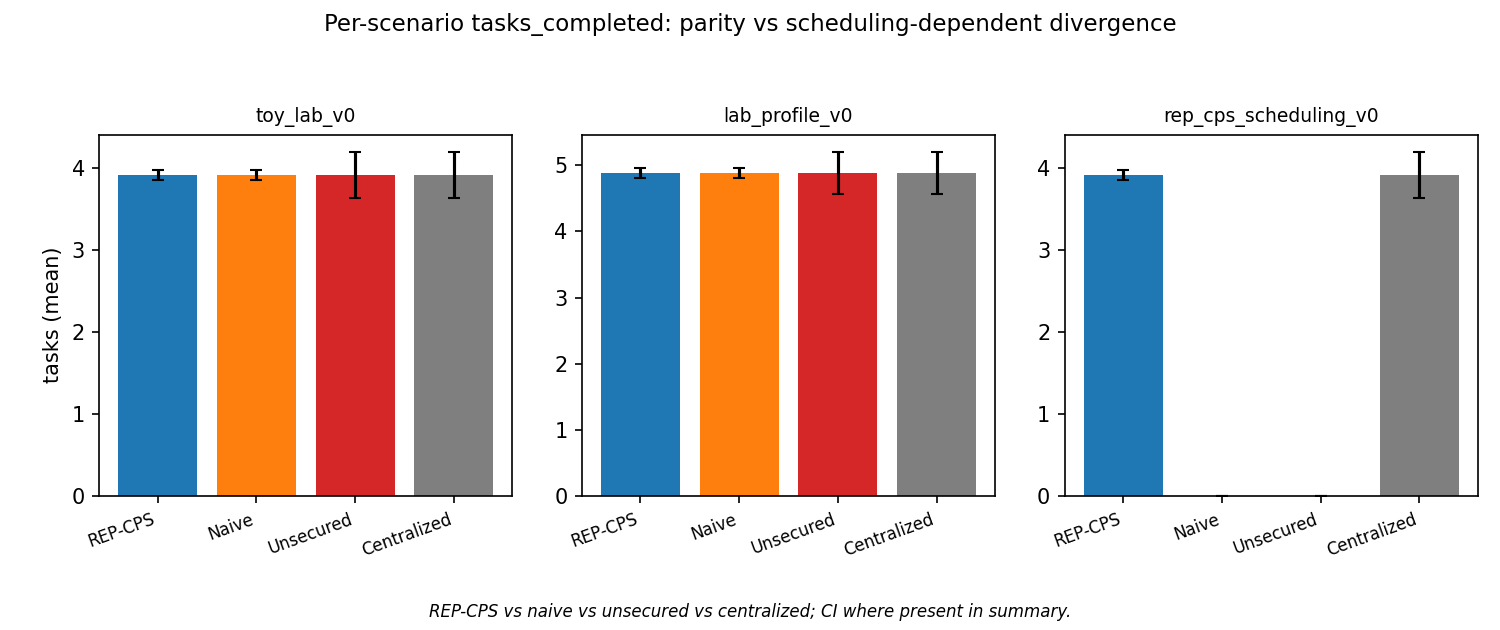
\includegraphics[width=\linewidth]{../../docs/figures/p2_rep_cps_tasks_per_scenario.png}
}{
    \fbox{\parbox[c][4.2cm][c]{\linewidth}{\centering Fig.~1a placeholder: per-scenario tasks.\\ \tool{plot\_rep\_cps\_summary.py}}}
}
\caption{Per-scenario tasks by policy (main operational read).}
\label{fig:tasks-scenario}
\end{subfigure}
\hfill
\begin{subfigure}[t]{0.48\linewidth}
\centering
\IfFileExists{../../docs/figures/p2_rep_cps_tasks.png}{
    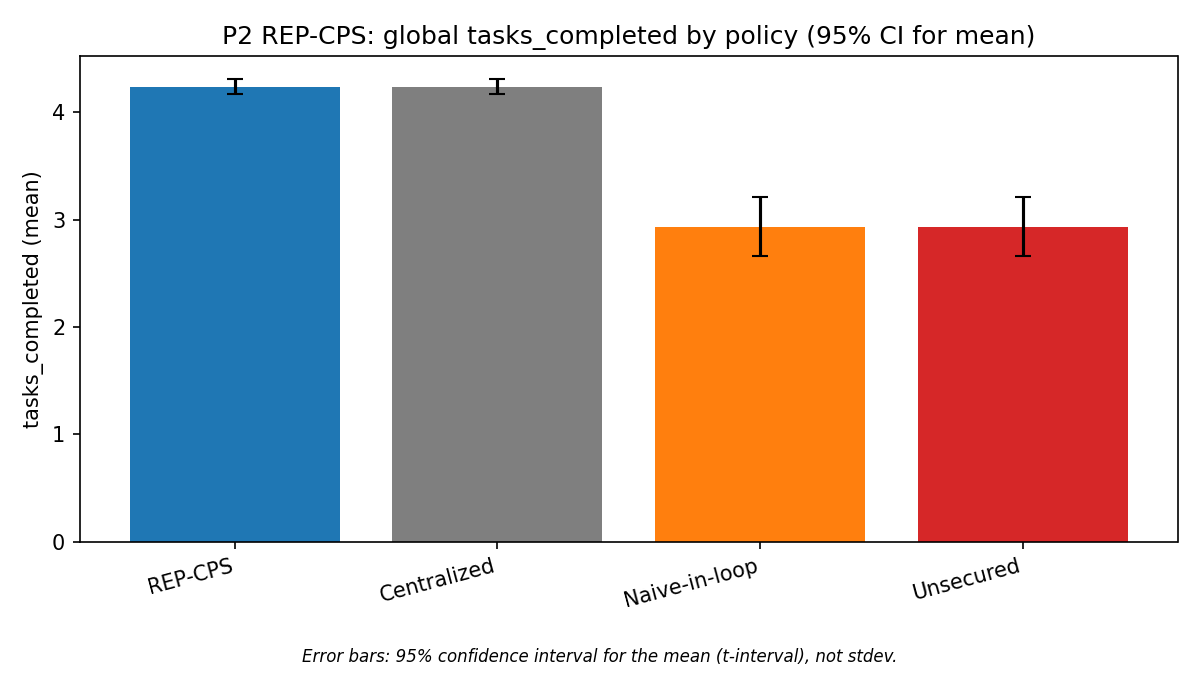
\includegraphics[width=\linewidth]{../../docs/figures/p2_rep_cps_tasks.png}
}{
    \fbox{\parbox[c][4.2cm][c]{\linewidth}{\centering Fig.~1b placeholder: global means.\\ \tool{plot\_rep\_cps\_summary.py}}}
}
\caption{Global policy means with 95\% CI for the mean (t-interval).}
\label{fig:tasks-global}
\end{subfigure}
\caption{Tasks completed: (a) separates parity scenarios from scheduling-dependent divergence where naive and unsecured paths collapse on \code{rep\_cps\_scheduling\_v0}; (b) global means blend scenarios and are secondary to (a) for the scheduling thesis.}
\label{fig:tasks}
\end{figure}

\begin{figure}[H]
\centering
\IfFileExists{../../docs/figures/p2_rep_cps_gate_threshold.png}{
    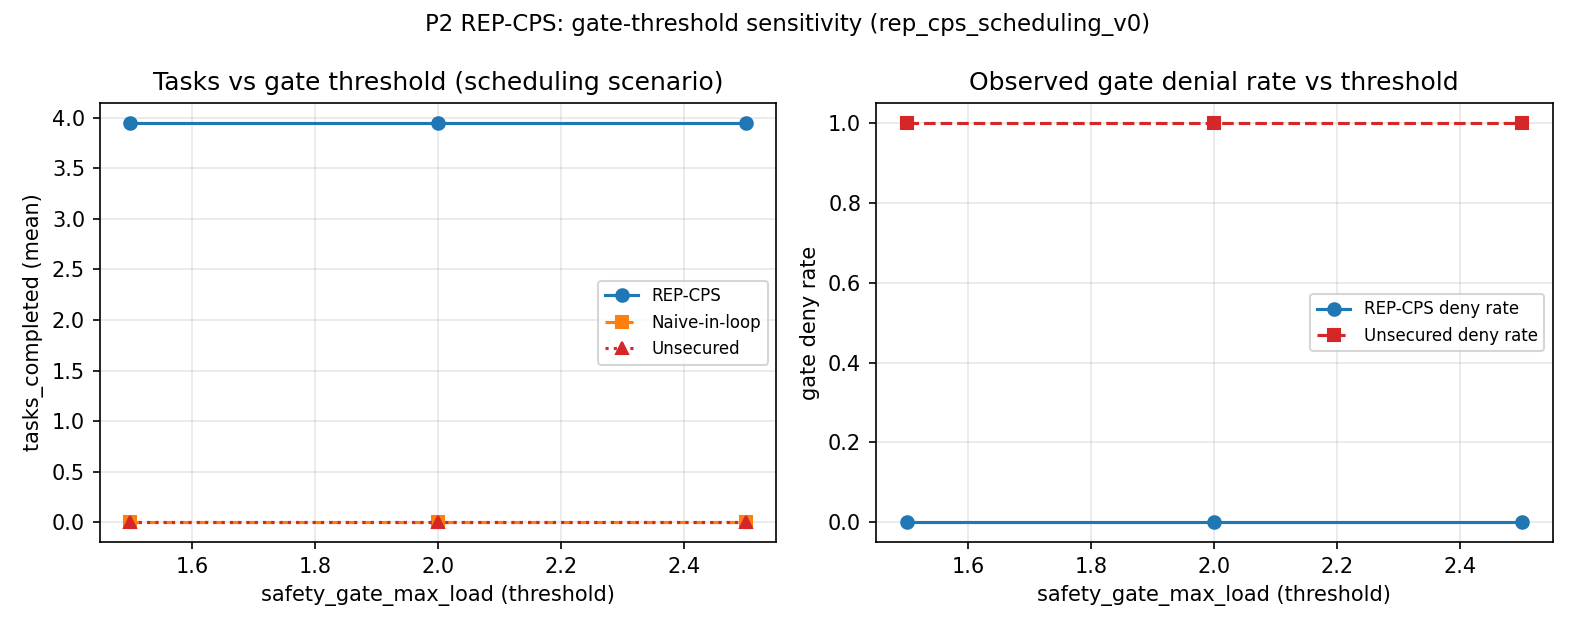
\includegraphics[width=0.92\linewidth]{../../docs/figures/p2_rep_cps_gate_threshold.png}
}{
    \fbox{\parbox[c][4cm][c]{0.92\linewidth}{\centering Figure 2 placeholder: gate-threshold sweep.\\Source: \tool{plot\_rep\_cps\_gate\_threshold.py} (requires gate sweep in \field{summary.json}).}}
}
\caption{Gate-threshold sensitivity on \code{rep\_cps\_scheduling\_v0}: tasks vs threshold (left) and observed deny rates (right). Naive and unsecured paths remain at zero tasks across the tested thresholds while \repcps{} remains admissible.}
\label{fig:gate}
\end{figure}

\begin{figure}[H]
\centering
\IfFileExists{../../docs/figures/p2_rep_cps_dynamics.png}{
    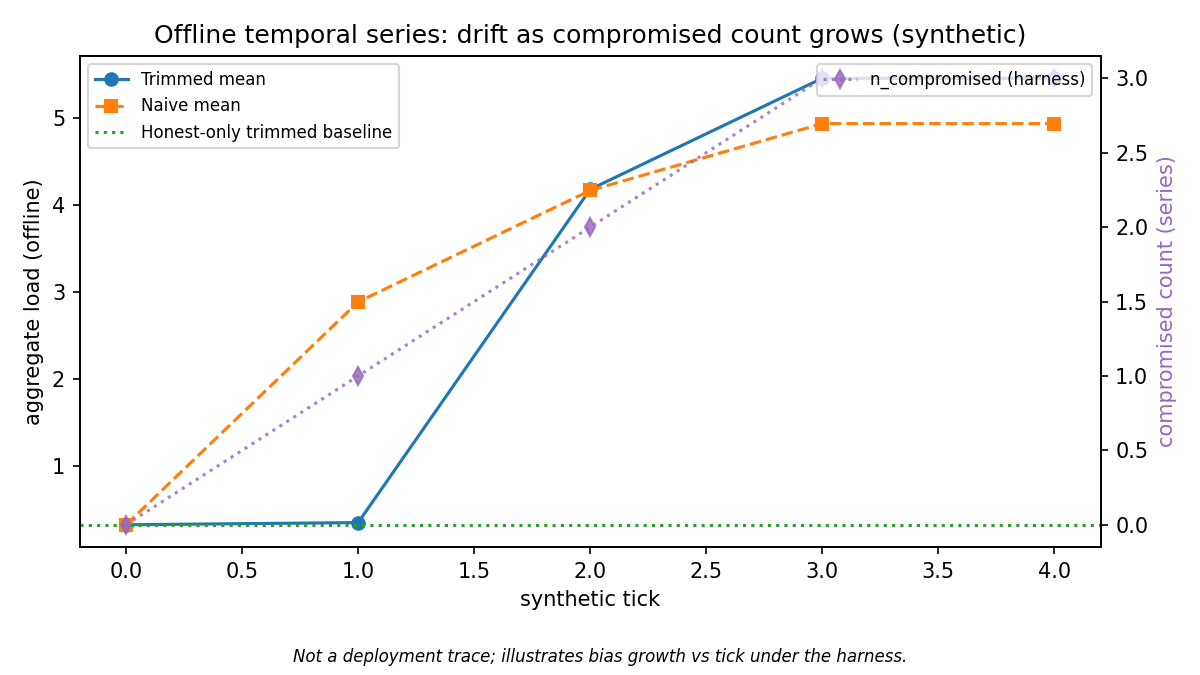
\includegraphics[width=0.88\linewidth]{../../docs/figures/p2_rep_cps_dynamics.png}
}{
    \fbox{\parbox[c][4cm][c]{0.88\linewidth}{\centering Figure 3 placeholder: dynamic series.\\Source: \tool{plot\_rep\_cps\_dynamics.py}.}}
}
\caption{Offline synthetic temporal series: trimmed mean vs naive mean vs honest-only baseline as compromised count increases by tick (harness, not a field trace). Supports the temporal subsection; does not prove long-run stability under all attacks.}
\label{fig:dynamics}
\end{figure}

\begin{figure}[H]
\centering
\IfFileExists{../../docs/figures/p2_rep_cps_latency.png}{
    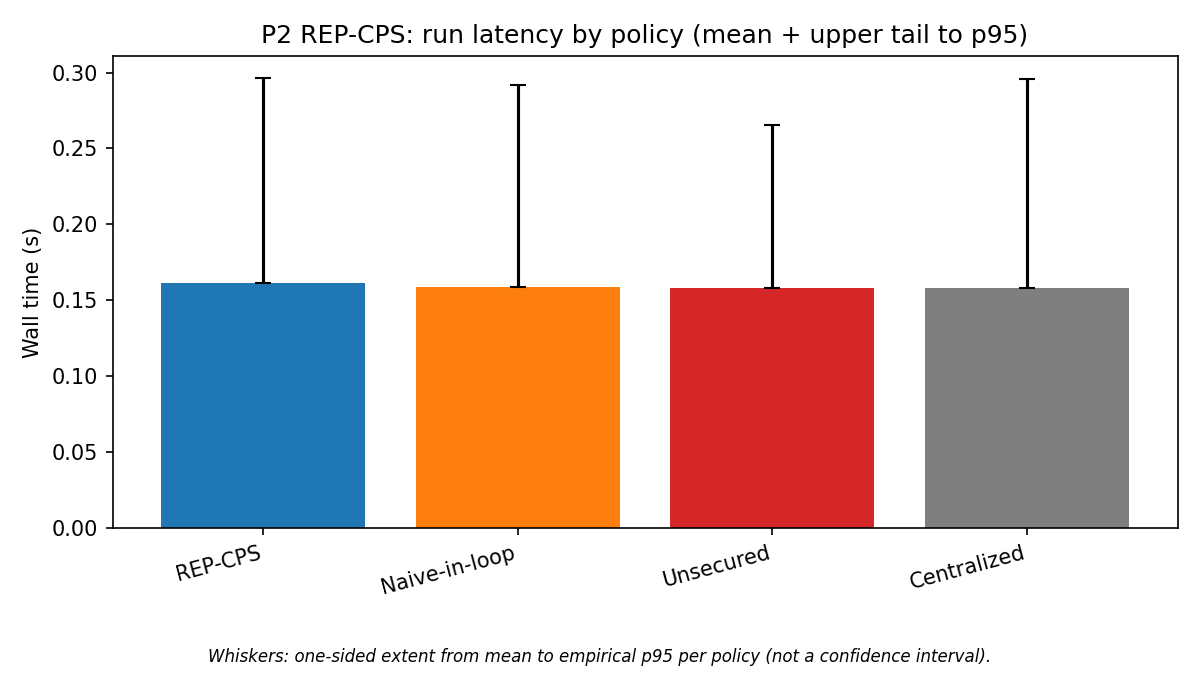
\includegraphics[width=0.78\linewidth]{../../docs/figures/p2_rep_cps_latency.png}
}{
    \fbox{\parbox[c][5cm][c]{0.78\linewidth}{\centering Figure 4 placeholder: latency by policy.\\Source: \tool{plot\_rep\_cps\_latency.py}.}}
}
\caption{Run latency by policy: bar height is mean wall time; whiskers extend to empirical p95 (one-sided tail, not a confidence interval). Overhead remains small relative to centralized execution on the measured workload.}
\label{fig:latency}
\end{figure}

\section{Discussion}

The most important outcome is not merely that 3.87 falls to 3.24 in the offline aggregation test. The broader result is that informational coordination channels in CPS should be treated as governed interfaces rather than informal side channels.

The paper also reveals an analytically useful boundary condition. On some architectures, robust aggregation changes the aggregate but not the mission outcome because the scheduler never consumes that informational state. On other architectures, such as \code{rep\_cps\_scheduling\_v0}, the same informational path becomes operationally relevant. This boundary is not a weakness of the paper; it is one of its primary scientific outputs.

\paragraph{Design principles.}
\begin{itemize}[leftmargin=1.5em]
    \item \textbf{P1:} Informational state is not harmless if it can shape action.
    \item \textbf{P2:} Admission controls are part of semantics, not preprocessing.
    \item \textbf{P3:} Aggregation robustness is insufficient without provenance and rate control.
    \item \textbf{P4:} Operational effect must be mediated explicitly.
    \item \textbf{P5:} Evaluation must separate offline robustness, in-loop bounded behavior, and operational effect.
\end{itemize}

\subsection{Portable takeaway for practitioners}

Readers who do not adopt \repcps{} verbatim can still reuse the checklist implied by the evidence model: (i) enumerate sensitivity variables that can influence scheduling or admission; (ii) specify admissibility (identity, freshness, rate) independently of the estimator; (iii) choose a bounded family of aggregators and record offline bias under compromise; (iv) ensure protocol output is informational and route any operational use through an explicit gate with traceable deny behavior; (v) report per-scenario outcomes when some paths are informational-only and others are scheduling-dependent. Portability is in the discipline and the evaluation methodology, not only in the trimmed-mean default.

\subsection{Deployment readiness checklist}
\begin{itemize}[leftmargin=1.5em]
    \item \textbf{Identity assumptions:} state enrollment and sender-identity trust roots; if Sybil resistance is absent, say so explicitly.
    \item \textbf{Freshness/rate policy:} define freshness windows and per-sender rate limits as semantic constraints, not optional preprocessing.
    \item \textbf{Gate calibration:} document threshold rationale, deny-rate expectations, and re-calibration triggers under workload drift.
    \item \textbf{Traceability:} retain denial traces and run manifests sufficient to reconstruct why gate decisions were made.
    \item \textbf{Negative-case testing:} include spoof, replay/staleness, burst influence, and compromised-value harness slices before deployment.
\end{itemize}

\subsection{Failure-mode playbook for repeated gate denials}
If repeated denials occur in a deployment-like setting, the operator path should be explicit: (i) confirm whether denials correlate with identity anomalies or stale/burst traffic; (ii) inspect aggregate composition and per-sender update rates; (iii) temporarily switch to a conservative fallback scheduling policy while preserving denial logs; (iv) re-evaluate gate thresholds only after identity/freshness policy verification; and (v) document post-incident changes in the profile manifest so future runs remain auditable.

\section{Limitations and threats to validity}

\paragraph{What the evidence establishes.}
The paper establishes that a profiled informational path can be implemented, attacked, ablated, and evaluated reproducibly; that robust aggregation reduces observed compromise-induced bias in the evaluated harness; that rate limits and other admission controls matter materially; and that gate-mediated informational state can change task outcomes on a scheduling-dependent scenario.

\paragraph{What the evidence does not establish.}
The paper does not establish a general Byzantine-resilience theorem, a Sybil-resistant identity architecture, a live distributed deployment, a real-time bounded-latency guarantee, or uniform operational benefit across all CPS architectures.

\paragraph{What would close the remaining gaps.}
A stronger operational paper would add a live messaging substrate, a scheduler that consumes the aggregate in richer ways than the current thin slice, stronger comparator families, and larger temporal studies with real deployment traces or an OPC UA-aligned integration path.

\paragraph{Threats to validity.}
\emph{Internal validity:} message generation is synthetic and scheduling linkage is explicit only on the scheduling-dependent scenario. \emph{External validity:} the scenario set is small and does not represent wide-area or production timing conditions. \emph{Construct validity:} metrics such as \field{aggregate\_load}, \field{bias\_robust}, and gate denial counts are proxies for bounded informational distortion rather than direct measurements of operational safety.

\section{Conclusion}

\repcps{} is a safety-gated deployment profile for authenticated sensitivity sharing in cyber-physical coordination. Its contribution is neither a new estimator nor a full operational deployment claim. Its contribution is a disciplined method for governing decision-relevant informational state: typed variables, admissibility controls, bounded aggregation, explicit gate mediation, and reproducible evidence. The paper shows when such a profile behaves better under compromise, when it remains throughput-neutral, and when it becomes operationally relevant. This is a more useful outcome than either an overclaimed positive paper or a purely defensive negative one.

\appendix

\section{Claim-to-evidence map}

\begin{table}[H]
\centering
\caption{Claim-to-evidence map for the paper.}
\label{tab:claims-map}
\begin{tabular}{p{1.1cm}p{8.4cm}p{4.0cm}}
\toprule
Claim & Statement & Primary evidence \\
\midrule
C1 & Deployable profile within evaluated assumptions. & Profile spec, Table~\ref{tab:overall}, Table~\ref{tab:ablation}, Table~\ref{tab:latency}, Figure~\ref{fig:profile} \\
C2 & Robust aggregation reduces compromise-induced bias; admission controls matter. & Table~\ref{tab:agg}, Table~\ref{tab:ablation}, Table~\ref{tab:envelope} \\
C3 & Protocol output is not directly actuating; gate mediation yields scoped task-level effect. & Theorem 1, Table~\ref{tab:scheduling}, Table~\ref{tab:safety} \\
C4 & Reproducible evaluation methodology. & Tables~\ref{tab:agg}--\ref{tab:envelope}, Figures~\ref{fig:profile}--\ref{fig:latency} \\
\bottomrule
\end{tabular}
\end{table}

\begin{thebibliography}{11}

\bibitem{dolev1986}
Danny Dolev, Nancy A. Lynch, Shlomit S. Pinter, Eugene W. Stark, and William E. Weihl.
\newblock Reaching approximate agreement in the presence of faults.
\newblock \emph{Journal of the ACM}, 33(3):499--516, 1986.

\bibitem{yin2018}
Dong Yin, Yudong Chen, Kannan Ramchandran, and Michael I. Jordan.
\newblock Byzantine-robust distributed learning: Towards optimal statistical rates.
\newblock In \emph{Proceedings of the 35th International Conference on Machine Learning (ICML)}, pages 5650--5659, 2018.

\bibitem{nistcps2017}
Edward A. Griffor, Chris Greer, David A. Wollman, and Martin Burns.
\newblock \emph{Framework for Cyber-Physical Systems: Volume 1, Overview}.
\newblock NIST Special Publication 1500-201, National Institute of Standards and Technology, 2017.

\bibitem{opclads2023}
OPC Foundation.
\newblock \emph{OPC UA for Laboratory and Analytical Devices (LADS), Version 1.00}.
\newblock Online reference specification, 2023.

\bibitem{alur2015}
Rajeev Alur.
\newblock \emph{Principles of Cyber-Physical Systems}.
\newblock MIT Press, 2015.

\bibitem{lee2017}
Edward A. Lee and Sanjit A. Seshia.
\newblock \emph{Introduction to Embedded Systems: A Cyber-Physical Systems Approach}.
\newblock MIT Press, 2017.

\end{thebibliography}

\end{document}
